\subsection[Il perceptron]{\textit{Il perceptron}}

\begin{frame}
	
	\frametitle{Il perceptron}

%	\begin{block}{}
		\begin{figure}[!htbp]
			\centering
			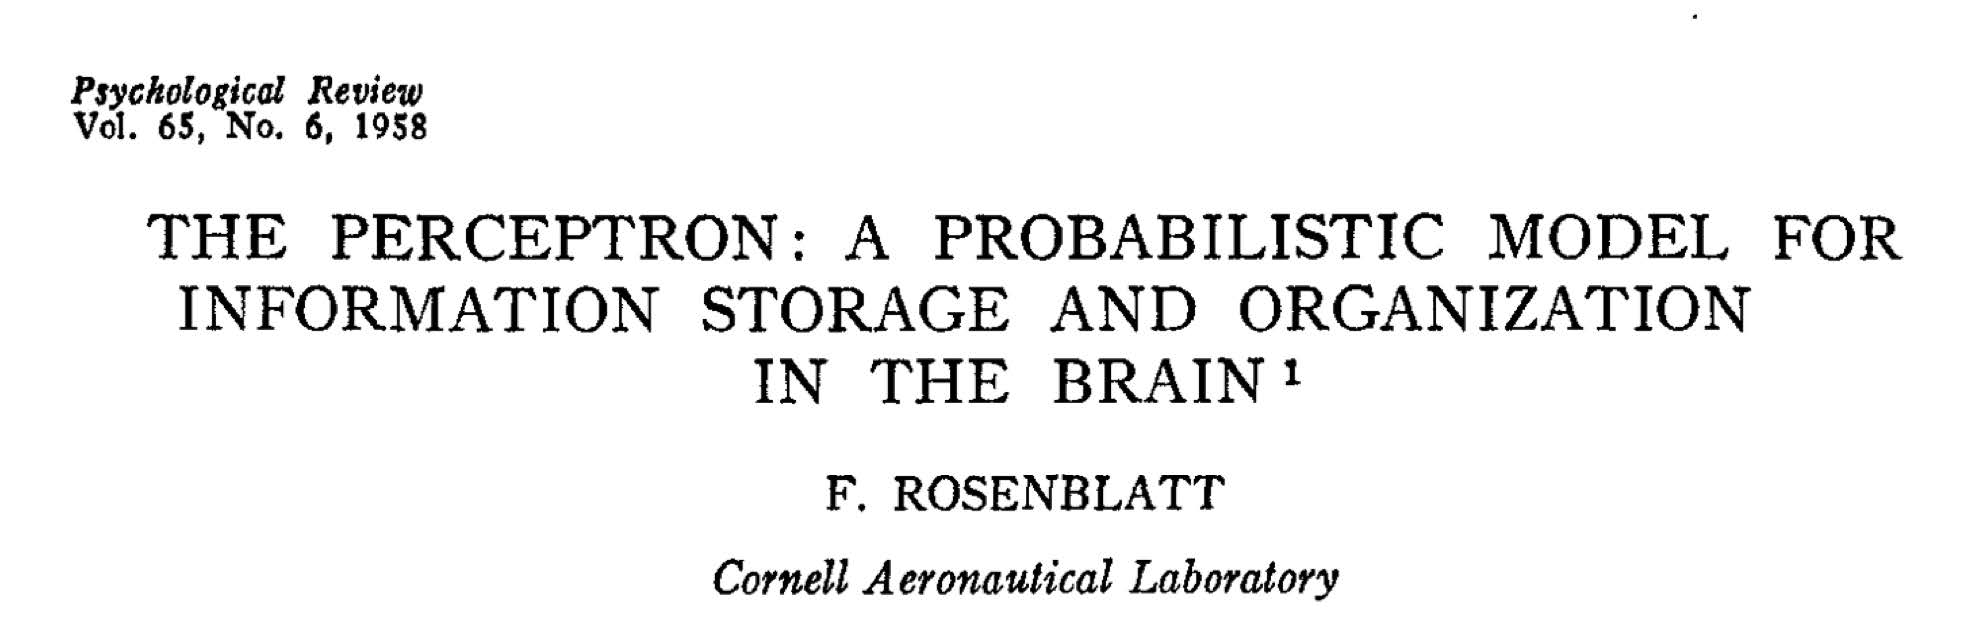
\includegraphics[width=1.0\linewidth]{images/supervised/perceptron/ronsenblatt_psychological_review.jpg}
			%\caption{Stripe Radar for Fraud Detection}
		\end{figure}
%	\end{block}

\end{frame}


\begin{frame}
	
	\frametitle{Il perceptron}
	
%	\begin{block}{}
		Fu \textbf{Frank Rosenblatt}, del \textit{Cornell Aeronautical Laboratory}, a ideare il \textbf{perceptron}, nel 1957 ne simulò il funzionamento su un IBM 704.\\
		%sotto gli auspici della United States Naval Research.\\
		Rosenblatt era uno psicologo, nonché pioniere nel campo dell'intelligenza artificiale. Assai competente di scienze cognitive, fu sua l'idea di creare un computer che potesse imparare attraverso prove ed errori, esattamente come un essere umano.
		\newlinedouble
		L'idea venne sviluppata con successo e, al principio, il perceptron non era stato concepito soltanto come un software, ma venne creato come software in esecuzione su un hardware dedicato.
		\newlinedouble
		Il perceptron, però, non fu in grado di realizzare le aspettative del suo creatore: ben presto dimostrò di avere \textbf{capacità limitate}, anche nella sua specializzazione, che era quella del riconoscimento di immagini.
		 
%	\end{block}

\end{frame}


\begin{frame}
	
	\frametitle{Il perceptron}
	
%	\begin{block}{}
		\begin{columns}
	
			\column{0.6\linewidth}
%			The New York Times, July 8 1958
			\begin{figure}[!htbp]
				\centering
				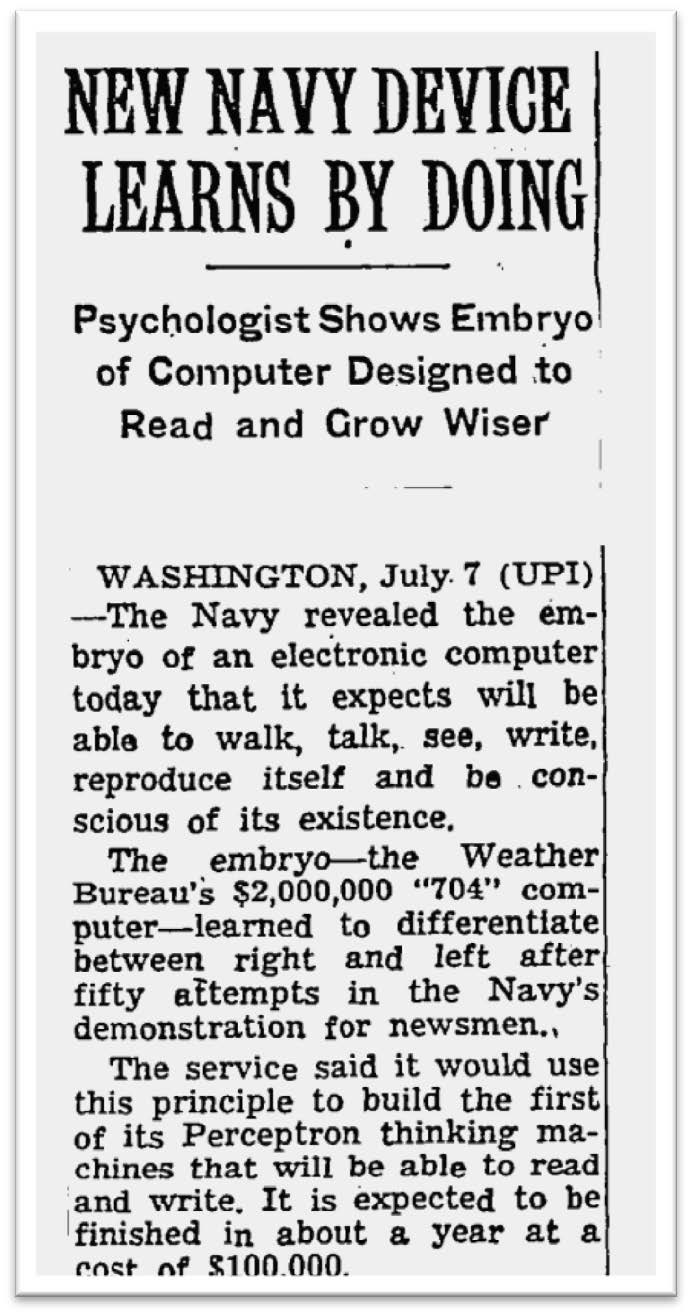
\includegraphics[width=0.46\linewidth]{images/supervised/perceptron/The_New_York_Times_July_8_1958.jpg}
				\caption{The New York Times, July 8 1958}
				%\label{Enel_QQ_Plot_Normal} 
			\end{figure}
			
			
			
			\column{0.4\linewidth}
			\begin{figure}[!htbp]
				\centering

				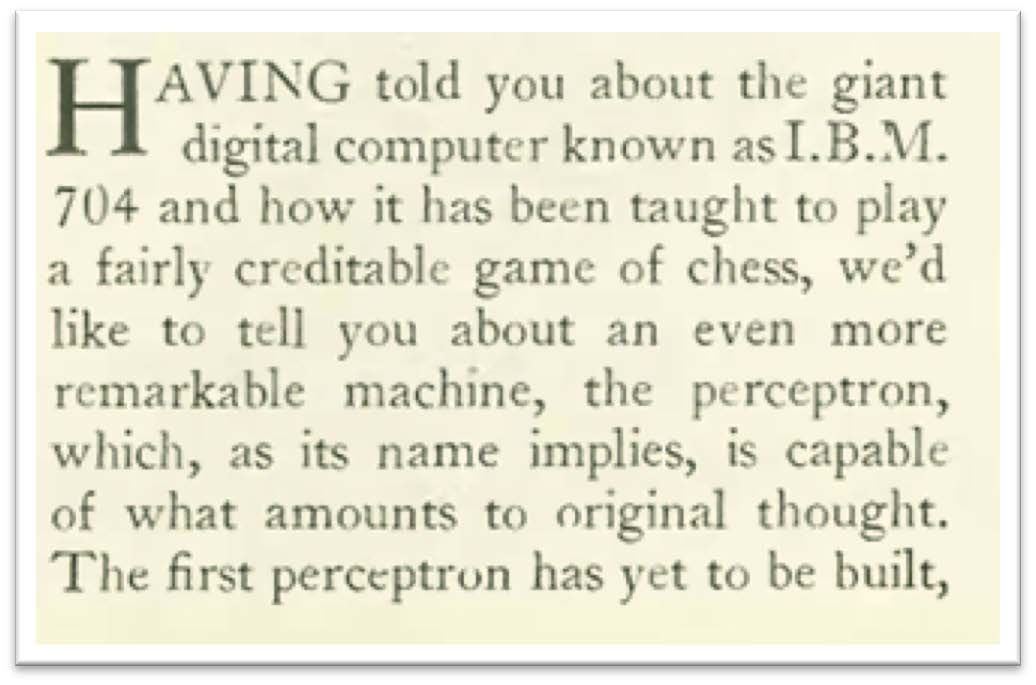
\includegraphics[width=1.0\linewidth]{images/supervised/perceptron/The_New_Yorker_December_6_1958_P44.jpg}
				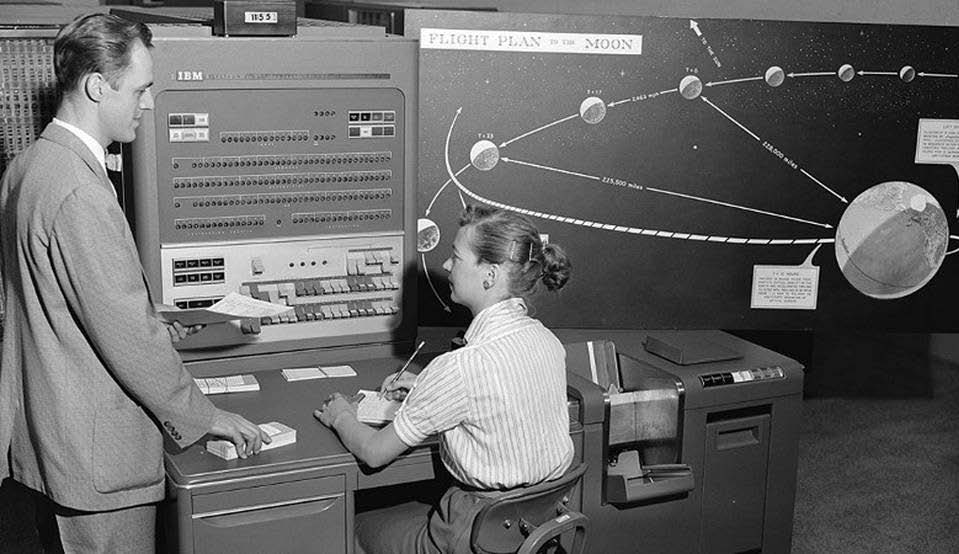
\includegraphics[width=0.8\linewidth]{images/supervised/perceptron/The_IBM_704_computer.jpg}
				\caption{The New Yorker, December 6, 1958 P. 44 sopra e l'IBM 704 sotto}
				%\label{Enel_QQ_Plot_Normal} 
			\end{figure}
			
		\end{columns}
		
%	\end{block}

\end{frame}


\begin{frame}
	
	\frametitle{Il perceptron}

%	\begin{block}{}
		Il perceptron è un algoritmo iterativo che tenta di determinare, per successive approssimazioni reiterate, il miglior insieme di valori per un vettore $\omega$, chiamato anche vettore dei coefficienti.
		\newlinedouble
		Il vettore $\omega$ può aiutare a prevedere la classe di un esempio quando lo si moltiplica per la matrice delle feature $X$, la quale contiene le informazioni in valori numerici, e quindi lo si somma a un termine costante, chiamato bias.
		\newlinedouble
		L'output è una previsione nel senso che le operazioni descritte in precedenza restituiscono un numero il cui segno dovrebbe essere in grado di prevedere con precisione la classe di ciascun esempio.\\
		Il perceptron, per sua natura, è specializzato nella classificazione binaria.
		
%	\end{block}

\end{frame}



\begin{frame}
	
	\frametitle{Il perceptron: un classificatore lineare}
	
%	\begin{block}{}
		\begin{itemize}
			\item input: un vettore $\underline{x}$ di dimensione $n$
			\item output: una label $\in \{-1, +1\}$
		\end{itemize}
		
		Come ogni classificatore lineare classifica un esempio $\underline{x}$ utilizzando la seguente regola di classificazione:
		\begin{itemize}
			\item output = $sgn(\underline{\omega}^T\underline{x} + b) = sgn( b + \sum\omega_i x_i )$
			\begin{itemize}
				\item[--] $\underline{\omega}^T\underline{x} + b \geq 0 \rightarrow$ predict $y = +1$
				\item[--] $\underline{\omega}^T\underline{x} + b < 0 \rightarrow$ predict $y = -1$
			\end{itemize}
			$b$ prende il nome di $bias$ (anche indicato come $\omega_0$)\\
			il vettore $[ \omega_1, \omega_2, \dots, \omega_n ]$ è la normale dell'iperpiano
		\end{itemize}
		
		
		\begin{figure}[!htbp]
			\centering
			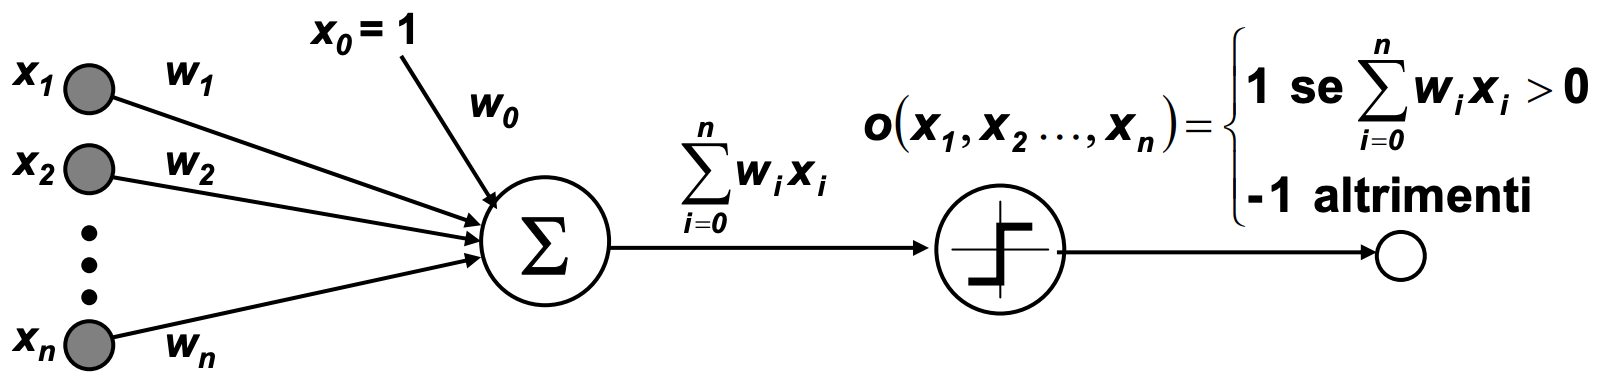
\includegraphics[width=1.0\linewidth]{images/supervised/perceptron/perceptron_formula.png}
			%\caption{Stripe Radar for Fraud Detection}
		\end{figure}
%	\end{block}

\end{frame}


\begin{frame}

	\frametitle{Il perceptron: un classificatore lineare}
	
%	\begin{block}{}
		\begin{figure}[!htbp]
			\centering
			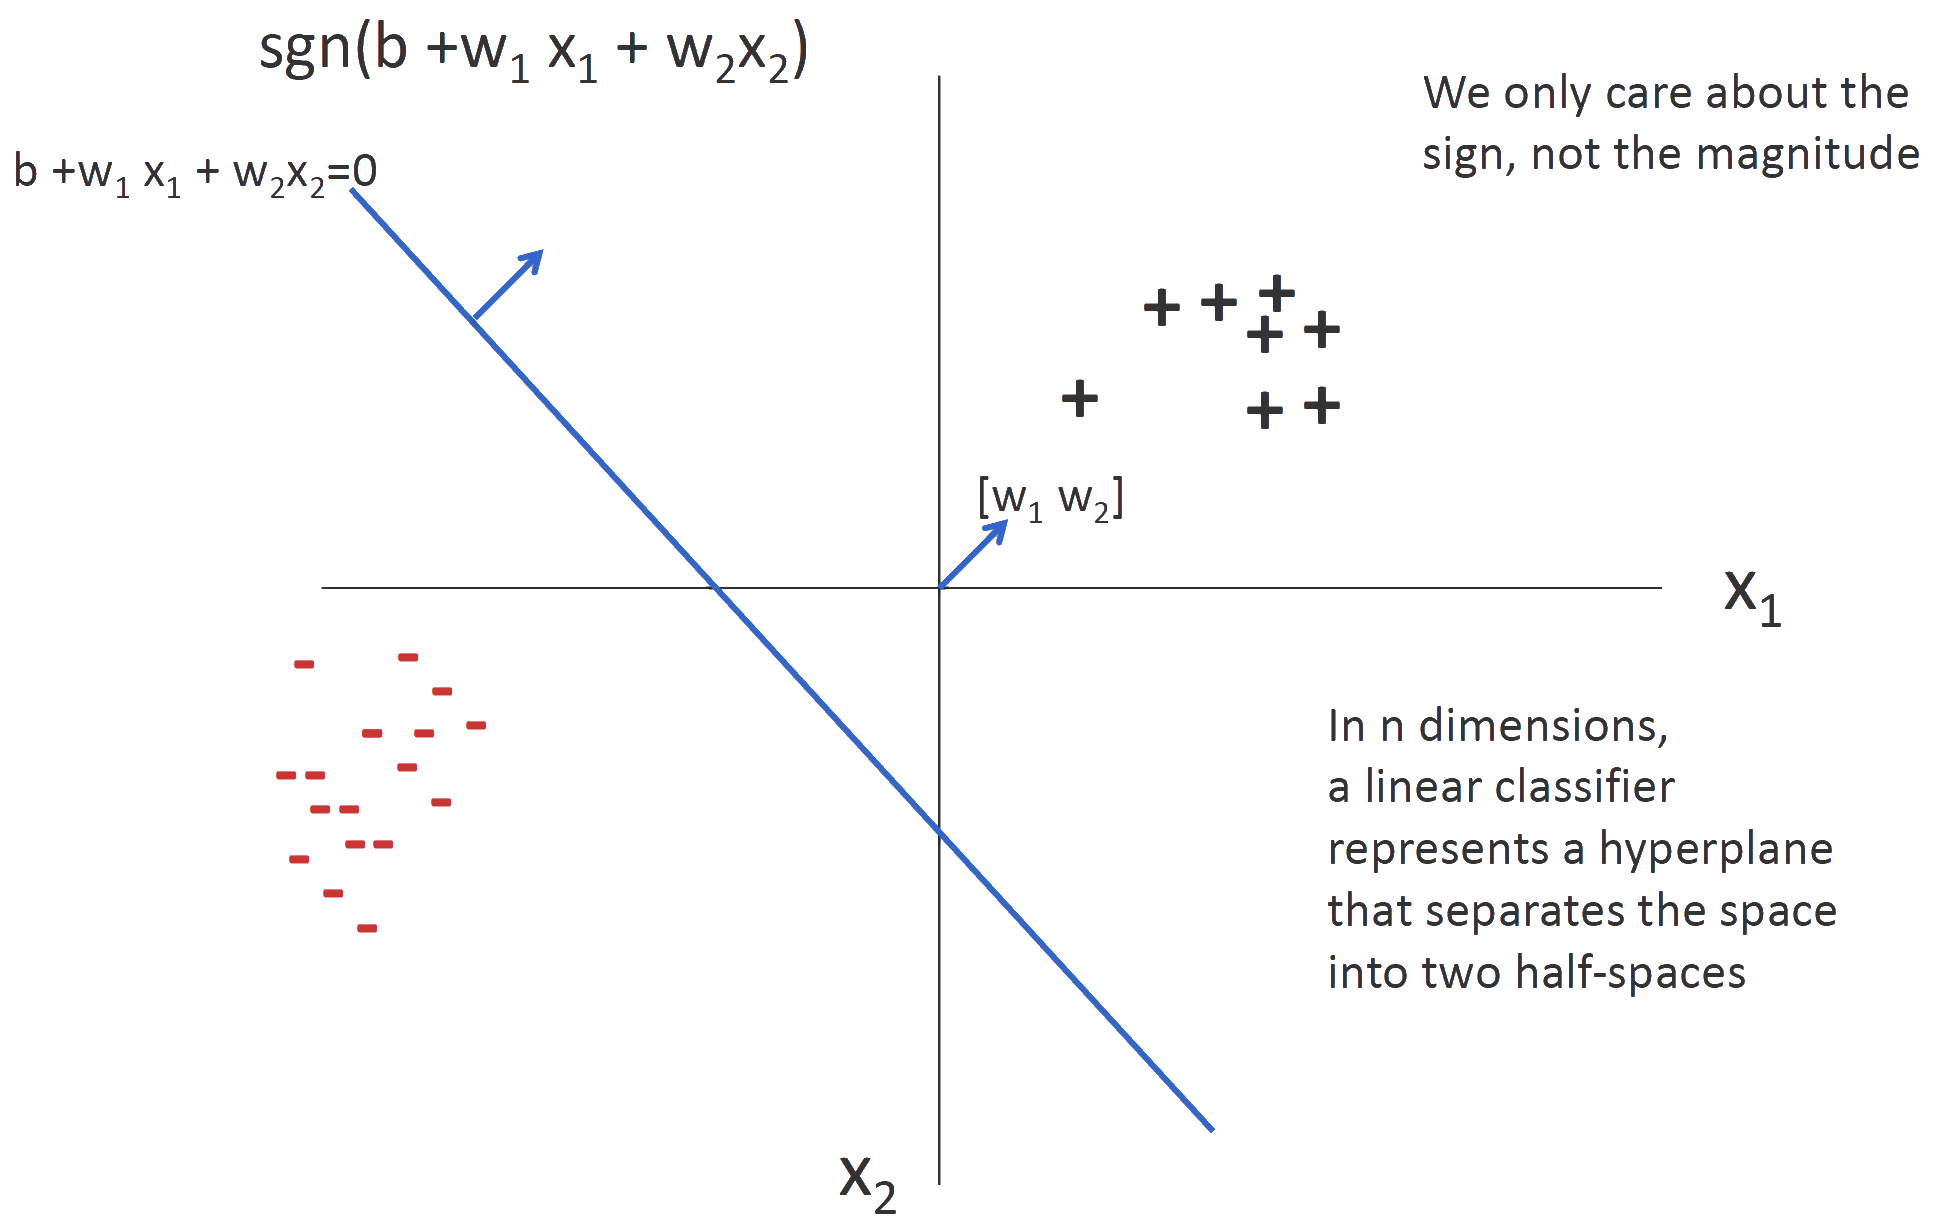
\includegraphics[width=1.0\linewidth]{images/supervised/perceptron/linear_classifier_1.png}
			%\caption{Stripe Radar for Fraud Detection}
		\end{figure}
%	\end{block}

\end{frame}


\begin{frame}
	
	\frametitle{Il perceptron: un classificatore lineare}
	
	\begin{itemize}
		\item<1-5> Si potrebbe vedere la linea blu come la funzione $\textcolor{blue}{y = -x -5}$.
		\item<2-5> Che riscriviamo usando $x_1$ e $x_2$ come: $\textcolor{blue}{x_2 = -x_1 - 5}$
		\item<3-5> Infine riportiamo il tutto in forma implicita: $\textcolor{blue}{5 + x_1 + x2 = 0}$
		\item<4-5> Quindi per questa retta (nel caso in cui avessimo avuto più dimensioni avremmo avuto un iperpiano) abbiamo $b = +5$, $\omega_1 = +1$, $\omega_2 = +1$
		\item<5> Testa con i punti: $(0,0), (-2,0), (-5,0), (0,-5), (0,-6)$
	\end{itemize}
	
%	\begin{block}{}
		\begin{figure}[!htbp] 
			\centering
			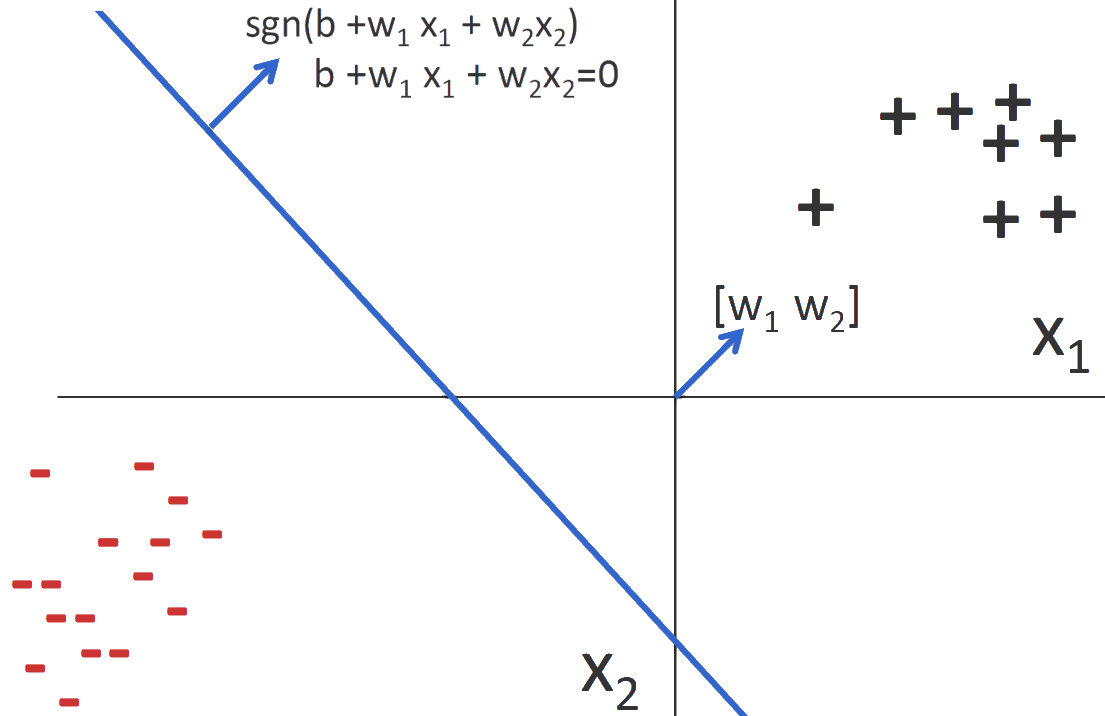
\includegraphics[width=0.55\linewidth]{images/supervised/perceptron/linear_classifier_2.png}
			%\caption{Stripe Radar for Fraud Detection}
		\end{figure}
%	\end{block}

\end{frame}


\begin{frame}
	
	\frametitle{Il perceptron}
	
	\begin{block}{L'algoritmo: intuizione geometrica}
	
		\begin{itemize}
			\item<1-3> nella figura di sinistra: l'iperpiano definito da $\omega_t$ classifica male un punto rosso (-1) e uno blu (+1)
			\item<2-3> nella figura nel centro: il punto rosso $x$ è scelto ed utilizzato per un aggiornamento. Poiché la sua label è -1 dobbiamo sottrarre $x$ a $\omega_t$
			\item<3> nella figura di destra: l'iperpiano aggiornato come $\omega_t = \omega_t-x$ separa le due classi e il perceptron quindi converge
		\end{itemize}
		
		\begin{figure}[!htbp]
			\centering
			\includegraphics<1>[width=0.6\linewidth]{images/supervised/perceptron/perceptron_algorithm_1.png}
			\includegraphics<2>[width=0.6\linewidth]{images/supervised/perceptron/perceptron_algorithm_2.png}
			\includegraphics<3>[width=0.6\linewidth]{images/supervised/perceptron/perceptron_algorithm_3.png}
			%\caption{Single-Link}
			%\label{Enel_HistFit_Normal}
		\end{figure}
		

	\end{block}

\end{frame}


\begin{frame}
	
	\frametitle{L'algoritmo: intuizione geometrica}
	
	%\begin{block}{}
		\centering
		\animategraphics[controls={play, step, stop}, height=7cm]{1.0}{images/supervised/perceptron/perceptron_algorithm_without_bias/perceptron_algorithm_without_bias-}{0}{32}
	%\end{block}

\end{frame}


\begin{frame}
	
	\frametitle{Il perceptron}
	
	\begin{block}{L'algoritmo}		
		\begin{figure}[!htbp]
			\centering
			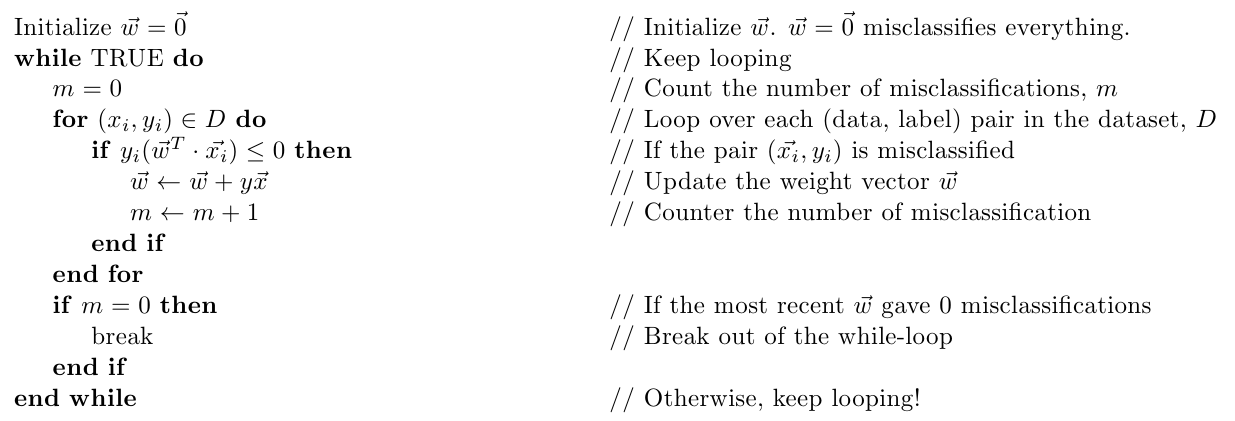
\includegraphics[width=1.0\linewidth]{images/supervised/perceptron/perceptron_algo.png}
			%\caption{Stripe Radar for Fraud Detection}
		\end{figure}

	\end{block}

\end{frame}


\begin{frame}
	
	\frametitle{Il perceptron: la convergenza del metodo}
	
%	\begin{block}{La convergenza del metodo}
	
		Il Perceptron è stato probabilmente il primo algoritmo con una forte garanzia formale.
		\textbf{Se un dataset è separabile linearmente, il perceptron troverà un iperpiano di separazione in un numero finito di aggiornamenti} (dimostrazione formale: \underline{\href{https://www.cs.cornell.edu/courses/cs4780/2018fa/lectures/lecturenote03.html}{Perceptron Convergence}}).
		\newlinedouble
		Tuttavia se i dati \textbf{non sono separabili linearmente, ciclerà per sempre}.\\
		Un esempio famoso di un semplice set di dati separabili non linearmente è lo XOR (Minsky 1969):
		\begin{figure}[!htbp]
			\centering
			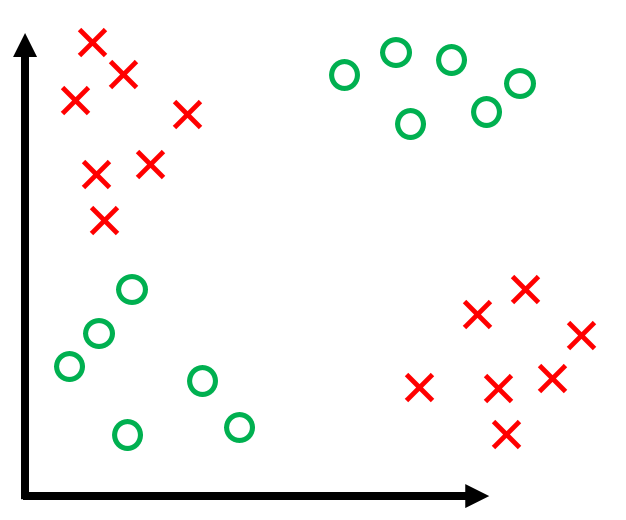
\includegraphics[width=0.35\linewidth]{images/supervised/perceptron/perceptron_xor.png}
%			\caption{}
		\end{figure}

		
%		\begin{figure}[!htbp]
%			\centering
%			\includegraphics[width=0.6\linewidth]{images/supervised/perceptron/perceptron_algorithm.png}
%%			\caption{}
%		\end{figure}

%	\end{block}

\end{frame}


\begin{frame}
	
	\frametitle{Il perceptron}
	
	\begin{block}{Una misura di errore del perceptron}
	
		Se indichiamo con $M$ l'insieme degli esempi classificati scorrettamente dal perceptron ad un certo step intermedio dell'algoritmo, potremmo usare la seguente formula per dare una misura dell'errore del perceptron:
		$$Error = -\sum_{i \in M} y_i(\underline{x_i}^T\underline{\omega}+b)$$
		che potremmo anche riscrivere come:
		$$Error = -\sum_{i \in D} \mathbb{I}[y_i(\underline{x_i}^T\underline{\omega}+b)<0]y_i(\underline{x_i}^T\underline{\omega}+b)$$
	\end{block}

\end{frame}


\begin{frame}
	
	\frametitle{Il perceptron}
	
	\begin{block}{Classificazione}
		
		Potremmo calcolare la classificazione durante l'esecuzione del perceptron per tutto il dataset $X$ come segue:
		$$\underline{\hat{y}} = sign(\doubleunderline{X}\text{ }\underline{\omega} + \underline{b})$$
	\end{block}
	
	\begin{block}{Aggiornamento con $\eta$}
		Nell'algoritmo visto si è assunto che il tasso di apprendimento $\eta$ fosse pari a 1.\\
		La formula più generica che tiene conto anche di un possibile tasso di apprendimento diverso è la seguente:
		$$\underline{\omega}=\underline{\omega} + \eta (\underline{x_i} y_i)$$
	\end{block}

\end{frame}


\begin{frame}
	
	\frametitle{Il perceptron: osservazioni}
	
%	\begin{block}{Osservazioni}
		\begin{itemize}
			\item<1-4> dà garanzie di convergenza qualora le classi siano linearmente separabili
			\item<2-4> non è adatto a lavorare con classi non linearmente separabili e il grande pubblico perse interesse in questo algoritmo
			\item<3-4> tale problema può essere risolto creando un nuovo spazio delle feature nel quale classi prima inseparabili diventano separabili
			\item<4> non ha la necessità di lavorare con tutti i dati in memoria, ma può tranquillamente utilizzare singoli esempi (aggiornando il proprio vettore dei coefficienti quando si rivela necessario a causa di un caso di classificazione errata)%. È pertanto l'algoritmo ideale da utilizzare per l'apprendimento online, per esempio quando è necessario apprendere da un esempio di big data alla volta
		\end{itemize}
		\begin{figure}[!htbp]
			\centering
			\includegraphics<2>[width=0.55\linewidth]{images/supervised/perceptron/kernel_trick_1.png}
			\includegraphics<3-4>[width=0.55\linewidth]{images/supervised/perceptron/kernel_trick_2.png}
%			\caption{}
		\end{figure}

%	\end{block}

\end{frame}



%\begin{frame}
%	
%	\frametitle{Classificazione di classi multiple: OvR e OvO}
%	
%%	\begin{block}{}
%		I problemi di classificazione \textbf{non sono sempre riconducibili a due classi} e quindi molti problemi di classificazione richiedono soluzioni che funzionino su risposte a classi multiple.\\
%		La maggior parte degli algoritmi che prevedono delle probabilità o un punteggio per le classi è in grado di gestire automaticamente i problemi di \textbf{classi multiple} utilizzando \textbf{due diverse strategie}:
%		\begin{itemize}
%			\item \textbf{One Versus Rest (OvR)}: l'algoritmo confronta ogni classe con quelle rimanenti, creando un modello per ogni classe. La classe con la probabilità più elevata è quella che viene scelta; pertanto, se un problema deve trovare tre classi, anche l'algoritmo utilizza tre modelli.
%			\item \textbf{One Versus One (OvO)}: in questo caso l'algoritmo compara a due a due le classi, creando un numero di modelli equivalente a $\frac{n(n-1)}{2}$, laddove $n$ è il numero delle classi. Quindi, se un problema ha cinque classi da predire, l'algoritmo One Versus One costruisce 10 modelli. 
%		\end{itemize}
%		
%%	\end{block}
%
%\end{frame}
